% Source: tex/chapters/ch05/11_ソフトウェアテストツール.tex
\subsubsection{ツールの分類}
代表的なツール分類を表に示す。

\par\smallskip\noindent\refstepcounter{table}\label{tab:ch05-03}\textbf{表 \thetable: 第05章 ソフトウェアテスト 表03}\par\smallskip
\begin{longtable}{P{0.27\linewidth}P{0.63\linewidth}}
\toprule
\textbf{分類} & \textbf{主な役割} \\
\midrule
テストハーネス & ドライバやスタブにより、部分的な SUT を制御された環境で実行し、出力を記録する。\\
テスト生成器 & ランダム、経路ベース、モデルベースなどによりテストケースを生成する。\\
キャプチャ・リプレイツール & 以前の入力や画面操作を記録し、再実行する。\\
オラクル・比較・表明検査ツール & 実行結果が成功かどうかの判定を支援する。\\
カバレッジ分析器・計測器 & プログラム中の文、分岐、経路などがどれだけ実行されたかを測る。\\
トレーサ & 実行経路の履歴を記録する。\\
回帰テストツール & 変更後の再実行、影響範囲に基づくテスト選択を支援する。\\
信頼性評価ツール & テスト結果を分析し、信頼性関連測度を可視化する。\\
注入ベースツール & 攻撃注入や欠陥注入により、特定条件での振る舞いを確認する。\\
シミュレーションベースツール & モデルを使ってシナリオを実行し、性質の検証や予測を行う。\\
セキュリティテストツール & 脆弱性、侵入、ファズテストなどを支援する。\\
テスト管理ツール & テスト計画、実行、データ収集、欠陥管理、報告を支援する。\\
クロスブラウザテストツール & 端末やブラウザごとに UI が期待どおり動くかを確認する。\\
負荷テストツール & 性能評価のために負荷を発生させ、関連データを集める。\\
欠陥追跡ツール & 欠陥報告、状態、修正履歴を管理する。\\
モバイルテストツール & 実機やエミュレータで、モバイルアプリの UI や動作を繰り返し確認する。\\
API テストツール & API の機能、性能、信頼性、セキュリティを自動テストする。\\
ウェブアプリケーションテストツール & ウェブベース SUT の機能、性能、利用者向け問題を確認する。\\
\bottomrule
\end{longtable}

\begin{figure}[htbp]
\centering
\IfFileExists{assets/fig-ch05-15.png}{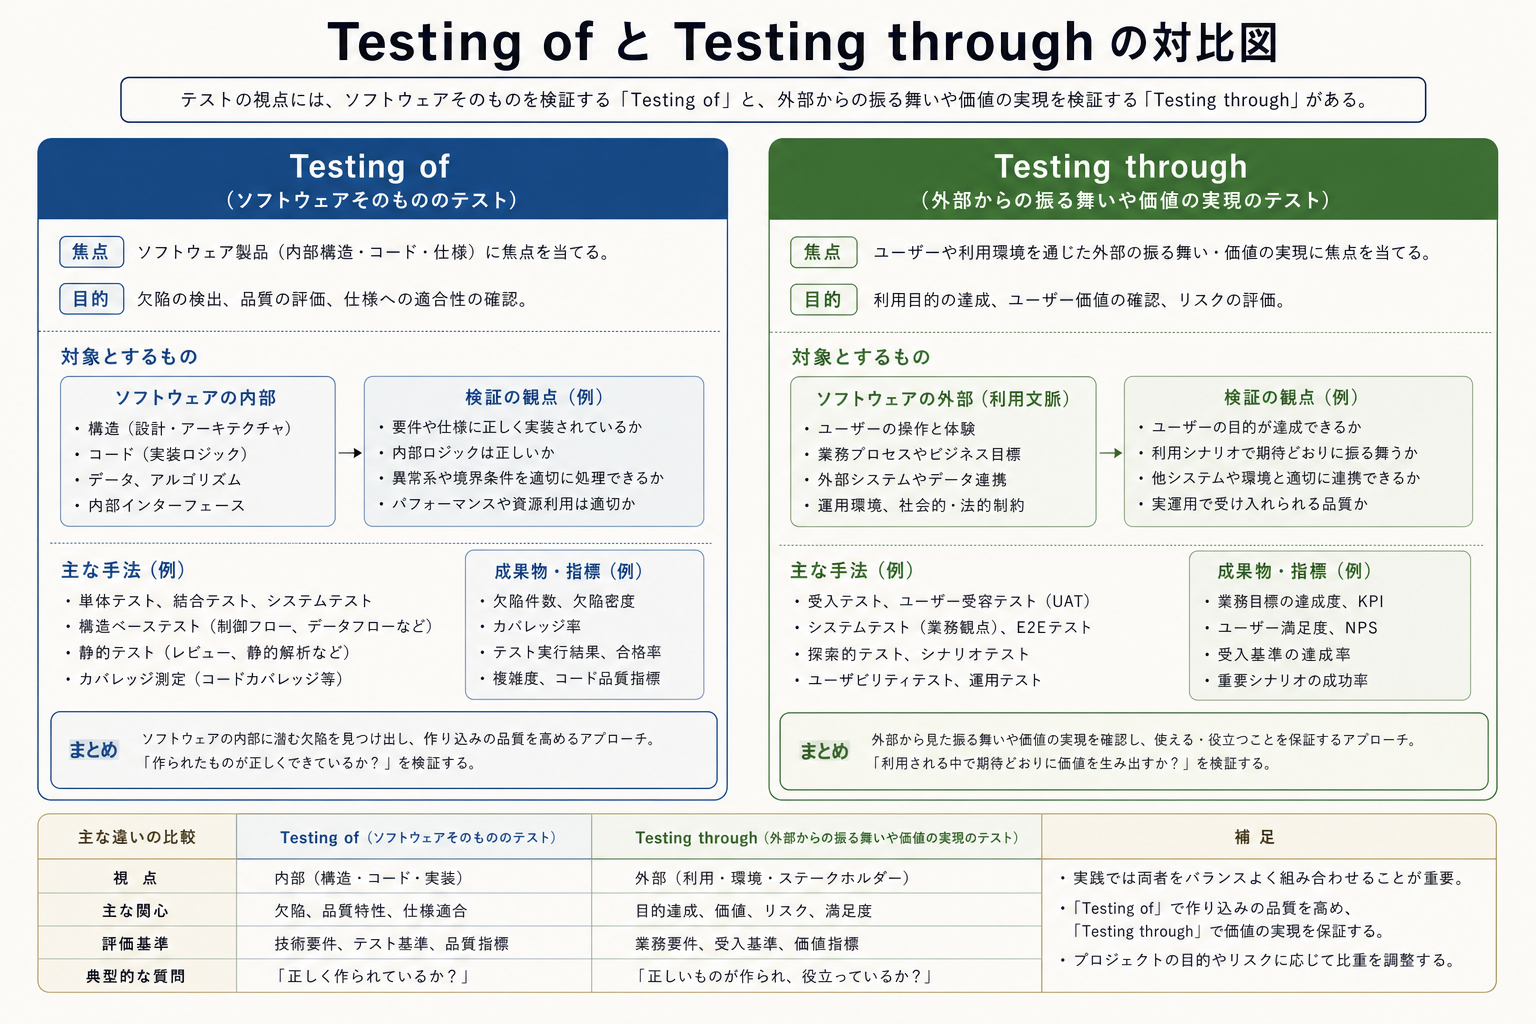
\includegraphics[width=0.96\linewidth]{assets/fig-ch05-15.png}}{\fbox{\parbox[c][48mm][c]{0.9\linewidth}{\centering 画像生成待ち\\テストツール分類図}}}
\caption{テストツール分類図}
\label{fig:ch05-15}
\end{figure}
